% Research status poster, A1 landscape (841 x 594 mm).
% Build: run poster\build.bat, or from this folder:  ..\tools\tectonic.exe poster.tex
% The plain-language flow figure is drawn by figures/make_simple_flow.py.
% No author or affiliation block, on purpose: several people contribute to this work.
% Every number comes from the repository (sources in poster/SOURCES.md); [TO FILL] marks
% what is not yet known.
\documentclass{article}
\usepackage[paperwidth=841mm,paperheight=594mm,margin=13mm]{geometry}
\usepackage[T1]{fontenc}
\usepackage{helvet}
\renewcommand{\familydefault}{\sfdefault}
\usepackage{xcolor,graphicx,tikz,enumitem,array,microtype}
\usetikzlibrary{arrows.meta,positioning}
\usepackage[hidelinks]{hyperref}
\hypersetup{pdftitle={Investigate, Fix or Escalate: research status poster},pdfauthor={},pdfsubject={Research status poster},pdfkeywords={}}

% The poster has no mathematics, but LaTeX still sets up maths fonts at each size. Tectonic's
% offline cache has only the 10 pt maths fonts, so scale those to every size.
\DeclareFontFamily{OT1}{cmr}{}\DeclareFontShape{OT1}{cmr}{m}{n}{<->cmr10}{}
\DeclareFontFamily{OML}{cmm}{\skewchar\font127}\DeclareFontShape{OML}{cmm}{m}{it}{<->cmmi10}{}
\DeclareFontFamily{OMS}{cmsy}{\skewchar\font48}\DeclareFontShape{OMS}{cmsy}{m}{n}{<->cmsy10}{}
\DeclareFontFamily{OMX}{cmex}{}\DeclareFontShape{OMX}{cmex}{m}{n}{<->cmex10}{}

\definecolor{navy}{HTML}{0B2E59}
\definecolor{alert}{HTML}{9B1111}
\definecolor{ink}{HTML}{111111}
\definecolor{tint}{HTML}{EAF0F7}
\definecolor{redtint}{HTML}{FBEAEA}

\pagestyle{empty}
\setlength{\parindent}{0pt}
\setlength{\parskip}{0pt}
\color{ink}

\newcommand{\body}{\fontsize{27}{33}\selectfont\raggedright\hyphenpenalty=10000\exhyphenpenalty=10000}
\newcommand{\head}[1]{%
  \par\noindent\colorbox{navy}{\parbox{\dimexpr\linewidth-2\fboxsep}{%
    \vspace{2mm}\color{white}\bfseries\fontsize{36}{42}\selectfont\hspace{2mm}#1\vspace{2mm}}}%
  \par\vspace{5mm}\body}
\newcommand{\gap}{\par\vspace{9mm}}
\setlist[itemize]{leftmargin=10mm,label={\color{navy}\rule[0.2ex]{0.55em}{0.55em}},itemsep=3mm,topsep=0mm,parsep=0mm}
\newcommand{\tbc}[1]{{\color{alert}\bfseries[#1]}}
\newcommand{\ra}{\tikz[baseline=-0.6ex]\draw[-{Latex[length=5mm,width=5mm]},line width=1.2mm,navy](0,0)--(11mm,0);}

\begin{document}
\raggedright\hyphenpenalty=10000\exhyphenpenalty=10000
% ------------------------------------------------------------------ title band
\noindent\colorbox{navy}{\parbox{\dimexpr\linewidth-2\fboxsep}{\centering\vspace{6mm}
  {\color{white}\bfseries\fontsize{64}{74}\selectfont Investigate, Fix or Escalate: A Rule-Constrained Reinforcement\\
   Learning Agent for IT Incident Triage under Ambiguous Evidence\par}
  \vspace{4mm}{\color{white}\fontsize{32}{38}\selectfont Research status, November 2026\par}\vspace{6mm}}}

\vspace{7mm}
% ------------------------------------------------------------------ three columns
\noindent
\begin{minipage}[t]{0.318\linewidth}
\head{1. Why this work}
When an IT problem is reported, its cause is often unclear. Staff must choose: look further, fix it, or pass it to a person. This work builds an assistant that learns that choice, with a separate rulebook check that blocks forbidden fixes.
\gap
\head{2. Literature review: how}
\begin{itemize}
\item \textbf{Databases:} Scopus, IEEE Xplore (open access), ACM Digital Library; 23 Oct 2026
\item \textbf{Method:} PRISMA 2020; Kitchenham and Charters procedure
\item \textbf{Appraisal:} eight-item checklist; synthesis around five questions
\item \textbf{Limit:} one AI-assisted screener; no citation searching yet
\end{itemize}
\vspace{7mm}
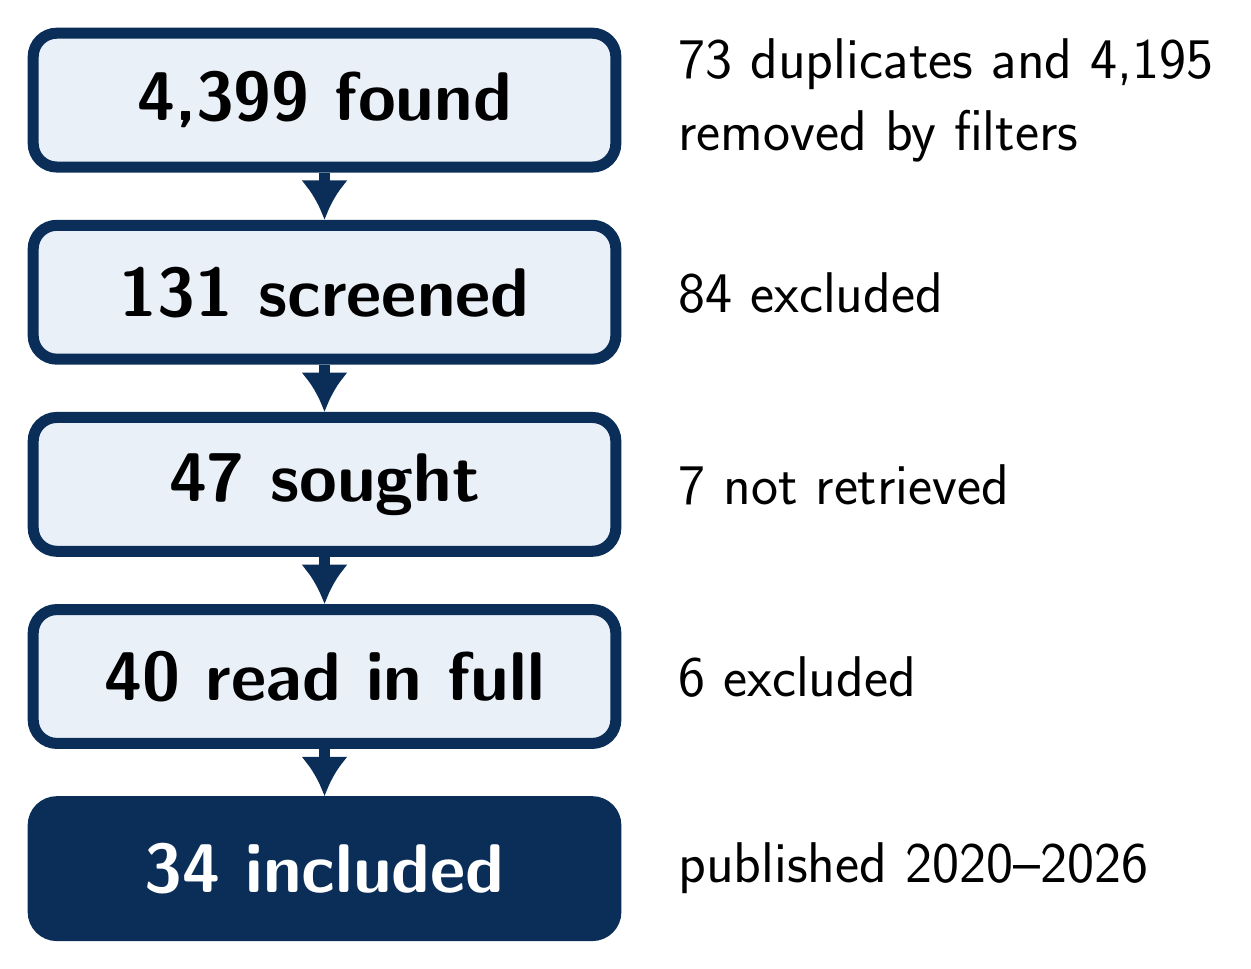
\begin{tikzpicture}[
  stage/.style={draw=navy,line width=1.4mm,fill=tint,rounded corners=3mm,minimum width=74mm,minimum height=17mm,align=center,font=\bfseries\fontsize{27}{31}\selectfont},
  note/.style={align=left,font=\fontsize{22}{26}\selectfont,anchor=west},
  arr/.style={-{Latex[length=5mm,width=6mm]},line width=1.4mm,navy}]
\node[stage] (a) {4,399 found};
\node[stage,below=6mm of a] (b) {131 screened};
\node[stage,below=6mm of b] (c) {47 sought};
\node[stage,below=6mm of c] (d) {40 read in full};
\node[stage,below=6mm of d,fill=navy,text=white] (e) {34 included};
\foreach \x/\y in {a/b,b/c,c/d,d/e} \draw[arr] (\x) -- (\y);
\node[note] at ([xshift=6mm]a.east) {73 duplicates and 4,195\\ removed by filters};
\node[note] at ([xshift=6mm]b.east) {84 excluded};
\node[note] at ([xshift=6mm]c.east) {7 not retrieved};
\node[note] at ([xshift=6mm]d.east) {6 excluded};
\node[note] at ([xshift=6mm]e.east) {published 2020--2026};
\end{tikzpicture}
\end{minipage}\hfill
% ------------------------------------------------------------------
\begin{minipage}[t]{0.318\linewidth}
\head{3. What the 34 studies show}
\begin{itemize}
\item \textbf{Hidden cause:} only 4 track what might be wrong
\item \textbf{Decisions:} 17 gather information, 7 pass to a person, 1 does all three
\item \textbf{Rules:} 5 use a hard block; only 3 say what happens to a blocked action
\item \textbf{Measures:} quality in 31, escalation in 5, rule-keeping in 4
\end{itemize}
\vspace{6mm}
\noindent\fcolorbox{alert}{redtint}{\parbox{\dimexpr\linewidth-2\fboxsep-1.2mm}{\vspace{3mm}\hspace{3mm}%
\parbox{\dimexpr\linewidth-6mm}{\raggedright{\color{alert}\bfseries\fontsize{32}{38}\selectfont Research gap\par}\vspace{2mm}
No study learns one policy that investigates, fixes or escalates IT service incidents under explicit rules.}\vspace{3mm}}}
\gap
\head{4. How the review shaped the pipeline}
{\renewcommand{\arraystretch}{1.15}\fontsize{23}{28}\selectfont
\begin{tabular}{@{}>{\raggedright\arraybackslash}p{0.42\linewidth}@{\hspace{3mm}}c@{\hspace{3mm}}>{\raggedright\arraybackslash}p{0.47\linewidth}@{}}
\textbf{Review found} & & \textbf{So this work} \\[2mm]
Unclear evidence rarely varied & \ra & Varies missing, wrong and overlapping evidence \\[3mm]
Passing on seldom learned & \ra & Makes it a choice with a cost \\[3mm]
Blocked actions unreported & \ra & Logs every block: one retry, then a person \\[3mm]
Escalation, rule-keeping rarely measured & \ra & Reports four groups of measures together \\[3mm]
Weak baselines, single runs & \ra & Strong baselines; several seeds \\
\end{tabular}}
\end{minipage}\hfill
% ------------------------------------------------------------------
\begin{minipage}[t]{0.318\linewidth}
\head{5. Dataset}
\begin{itemize}
\item \textbf{No tickets or personal data in training:} a scenario model that IT staff fill in through a workbook
\item \textbf{Pilot:} 8 causes, 11 checks, 4 symptoms, 5 rules, from one software developer
\item \textbf{Planned:} about 15 causes, 20 checks, 10 rules \tbc{TO FILL: elicitation date}
\item \textbf{Simulated tests:} 5,000 incidents never seen in training
\item \textbf{Prototype:} 8 fictional tickets; 20 sample tickets kept private \tbc{TO FILL: reader accuracy}
\end{itemize}
\gap
\head{6. Methodology}
\begin{itemize}
\item \textbf{Design and evaluate,} entirely in simulation
\item \textbf{Agent:} deep Q-network; \textbf{rulebook:} one retry, then a~person
\item \textbf{Compared with} 4 fixed, non-learning policies and 2 agents without the rulebook
\item \textbf{Four experiments:} baselines, rulebook effect, choices removed, worse evidence
\end{itemize}
\gap
\head{7. Status}
\begin{itemize}
\item \textbf{Done:} review; pilot simulator, rulebook and agents; Experiments 1--2 (3 seeds); working prototype
\item \textbf{Next:} full scenario model; 10 seeds; Experiments 3--4
\end{itemize}
\end{minipage}

% ------------------------------------------------------------------ plain-language flow
\vfill
\head{How the system works}
\vspace{-1mm}
\noindent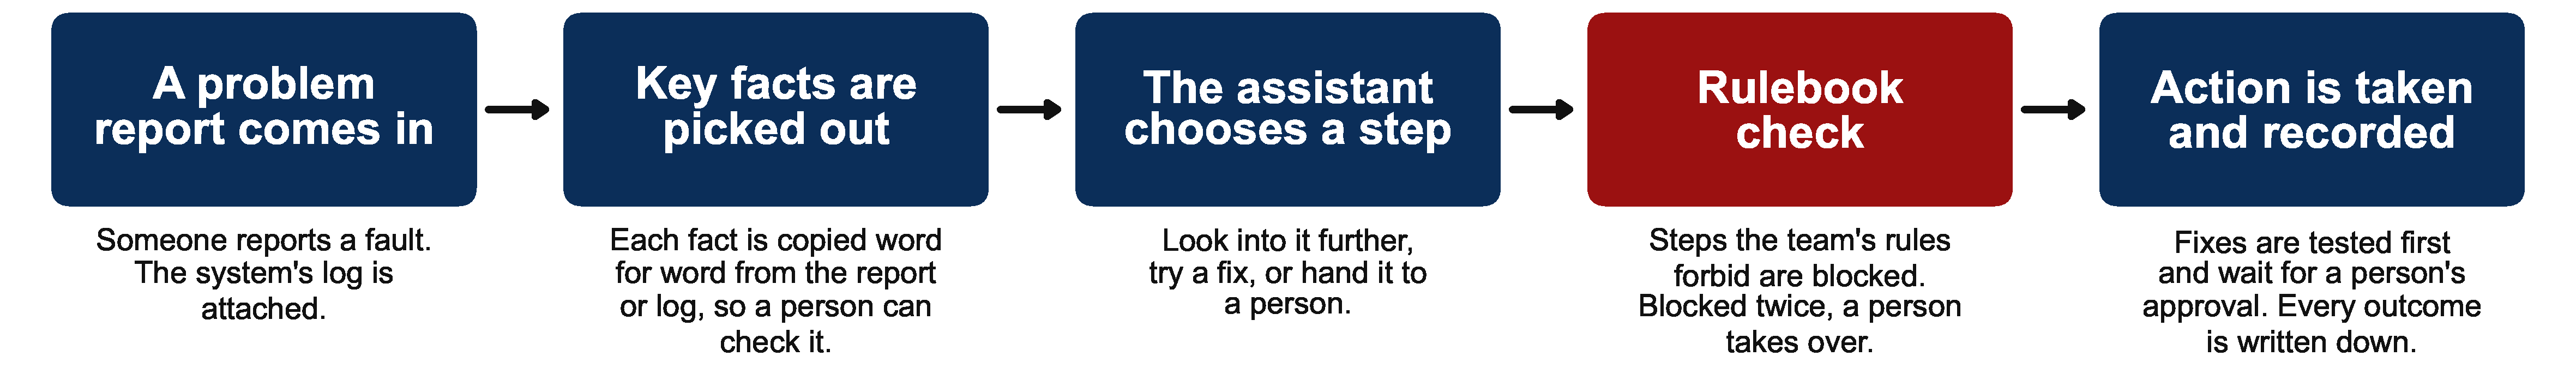
\includegraphics[width=\linewidth]{figures/simple_flow.pdf}

{\fontsize{18}{22}\selectfont\color{ink!75}
References: M. J. Page et al., \emph{BMJ}, 2021 (PRISMA 2020).\enspace
B. Kitchenham and S. Charters, EBSE-2007-01, 2007.\enspace
A. R. Hevner et al., \emph{MIS Quarterly}, 2004.\enspace
M. Alshiekh et al., AAAI, 2018.\par}
\end{document}
